\documentclass{article}
\usepackage{graphicx}
\renewcommand{\baselinestretch}{1}
\setlength{\textheight}{9in}
\setlength{\textwidth}{6.5in}
\setlength{\headheight}{0in}
\setlength{\headsep}{0in}
\setlength{\topmargin}{0in}
\setlength{\oddsidemargin}{0in}
\setlength{\evensidemargin}{0in}
\setlength{\parindent}{.3in}
\graphicspath{{images/}}

\title{Communication Systems \\
     \large Chapter 1 Introduction}
\author{Hunter Mills}
\date{\today}

\begin{document}
     \maketitle

     \begin{figure}[h]
     \centering
     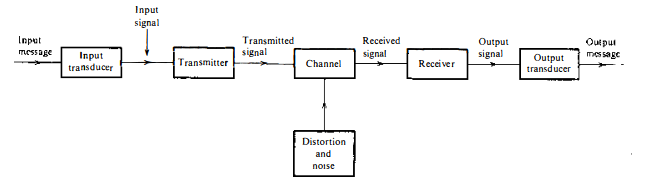
\includegraphics[width=0.75\textwidth]{bd}
     \caption{Comm Systems Block Diagram}
     \end{figure}

     \medskip
     Chapter 1 (Introduction) of Modern Digital and Analog Communication Systems.

     \section{Communication Systems}
     Figure 1 shows an example block diagram including common blocks.

     \begin{itemize}
          \item \textbf{Source}        - Originates the message (voice, picture) and if not an electrical signal uses an input transducer to convert to signal
          \item \textbf{Transmitter}   - Transforms the input signal into an appropriate for for efficient transmission. Can include a ADC, encoder and modulator.
          \item \textbf{Channel}       - The medium of choice that can convey the signal over a distance (coax, air).
          \item \textbf{Receiver}      - Similar to the transmitter, but reversing the signal transformation and removing the channel distortions. 
                                             Can include a DAC, decoder and demodulator.
     \end{itemize}

     \section{Channel Distortions and Noise}
     The channel is the physical medium between the transmitter and receiver. It acts as an imperfect filter attenuates and distorts the message. Some other 
     distortions can come from multi-path effects and Doppler shift. For example, a square wave will be smeared out in a channel that acts as a LPF. This is called
     \textbf{linear distortion} and can be partly corrected with an equalizer. In the channel \textbf{noise} (random variable) also affects the waveform.

     \section{Channel Effect, SNR, and Capacity}
     \subsection{Signal Bandwidth and Power}
     In a communication system, the fundamental parameters and physical limitations are the \textbf{channel bandwidth} ($B$) and the \textbf{$P_s$}. The bandwidth of 
     the channel is the range of frequencies that it can carry with reasonable fidelity. The \textbf{signal power} ($P_s$) is related to the quality of transmission.
     Increasing $P_s$ strengthens the signal and suppresses the channel effects (Increases the SNR). 

     \subsection{Channel Capacity and Data Rate}
     The SNR and Bandwidth of a signal effect the throughput of the communication system. The peak throughput that can be reliably carried by a channel is the
     channel capacity. A common channel is the additive white Gaussian noise (AWGN) channel and it assumes no channel distortions except for the additive white noise.
     The Shannon Channel Capacity is

     \begin{equation}  
          C = B \log_2 (1 + SNR) \quad \textrm{bits/s}
     \end{equation}

     The channel capacity $C$ is the upper bound of the transmission rate. It is impossible to transmit at a higher rate than $C$ without having very large
     numbers of bit errors. Practical systems operate much lower than $C$ since the tx/rx would be very complex.

     \section{Randomness, Redundancy and Source Coding}
     A message contains information only if it is unpredictable. Higher predictability means higher redundancy and less information. More unpredictable or less
     likely random signals contain more information. Source coding reduces redundancy based on the predictability of the message source. 

     \end{document}